% !TeX spellcheck = de
\chapter{Einleitung}
\label{sec:intro}

Im weiteren Verfahren soll an dem oben genannten Register-Client der dort angeschlossene RFID Chip-Kartenleser über geeignete Software in Betrieb genommen und die eingelesenen Daten an den Server übermittelt werden. Dafür wird ein Raspberry Pi verwendet, der zählt zu den beliebtesten Single Board Computern zält und lässt die andere Schnittstellen anzubinden. Der kompakter Einplatinencomputer wenig verbraucht Strom aber dennonch genügend Power für ein Linuxbetriebsystem liefert. 

\section{Ziel der Arbeit}
\label{sec:intro:goal}
Ziel dieser Arbeit ist die Entwicklung einer Datenbank-Applikation zur Verwaltung des Prozess von Ausleihe und Rückgabe der Hardware den Studentinnen und Studenten der Beuth Hochschule für Technik Berlin. Seit Jahren werden alle verknüpften mit der Ausleihverwaltung handlich verwaltet, was führt zum großen Arbeitszeitverbrauch. Obwohl das Thema der Bachelorarbeit "Entwicklung eine Datenbank-Applikation" lautet, besteht sie nicht nur aus einziger Aufgabe. sondern auch aus drei verteilte Teilen:
\begin{itemize}
\item Erstens wird an einem uComputer ein sogenannten Register-Client realisiert. Dafür ein RFID-Leser an uComputer angeschlossen wird. Register-Client ist neben dem Eingangstür eines kleinen Lagerraums des PSE-Labors zu platzieren ist, wo Raspi-Boards aufbewahrt werden. Es ist geplant, dass Studierende einen Board selbst aus dem Fach nehmen könnte und dann mit Hilfe des Register-Clients den genommenen Board auf sich oder seine Gruppe registrieren lassen. Der Register-Client hat selbst keinen Zugriff zur Datenbank und sollte nur die abgelesene Daten von der Smartcard der Studierende zur Server schicken. 
\item Zweitens ist ein Display-Client zu entwickeln, der den Studierenden es zulässt, die Begrüßung des System und eine Beschreibung die für Ausleihe notwendigen Schritten zu sehen. Es sollte in einem Browser-Fenster die aktuelle Server-Kommunikation und Auskunft angezeigt wird, ob die Ausleihe gelang oder ein Fehler aufgetreten war. Ein Android/iOS-Tablett ist eine gute Wahl für die technische Realisierung, da es die Kommunikation zwischen den Mensch und das System leicht und ohne erweiterte Hinweise zulässt. 
\item Drittens ist ein Web-Server für die Datenbank-Applikation schließlich zu implementieren. Er umfasst alle Datensätze über die vorhandenen im Labor Raspi-Boards, registrierten zum Kurs Studierenden und die abgewickelten Leihvorgänge.  Web-Server wird mit einem Web-Framework Django erstellt. Django verfügt nun über die Funktionalität und Datenbasis, um die dafür erforderlichen Aktionen durchzuführen. Als Web-Framework bietet Django eine Reihe von Komponenten und Funktionen (Benutzerauthentifizierung, Hochladen von Dateien, Umgang mit Daten usw.), die bei jeder Webanwendungen benötigt werden. Mit einem Web-Framework muss ein Entwickler keine Zeit damit verschwenden, denselben Code von Grund auf neu jedes Mal zu schreiben.
\end{itemize}

\section{Motivation und Aufgabestellung}
\label{sec:intro:motivation}
\begin{wrapfigure}{l}{0.4\textwidth}
	\fbox{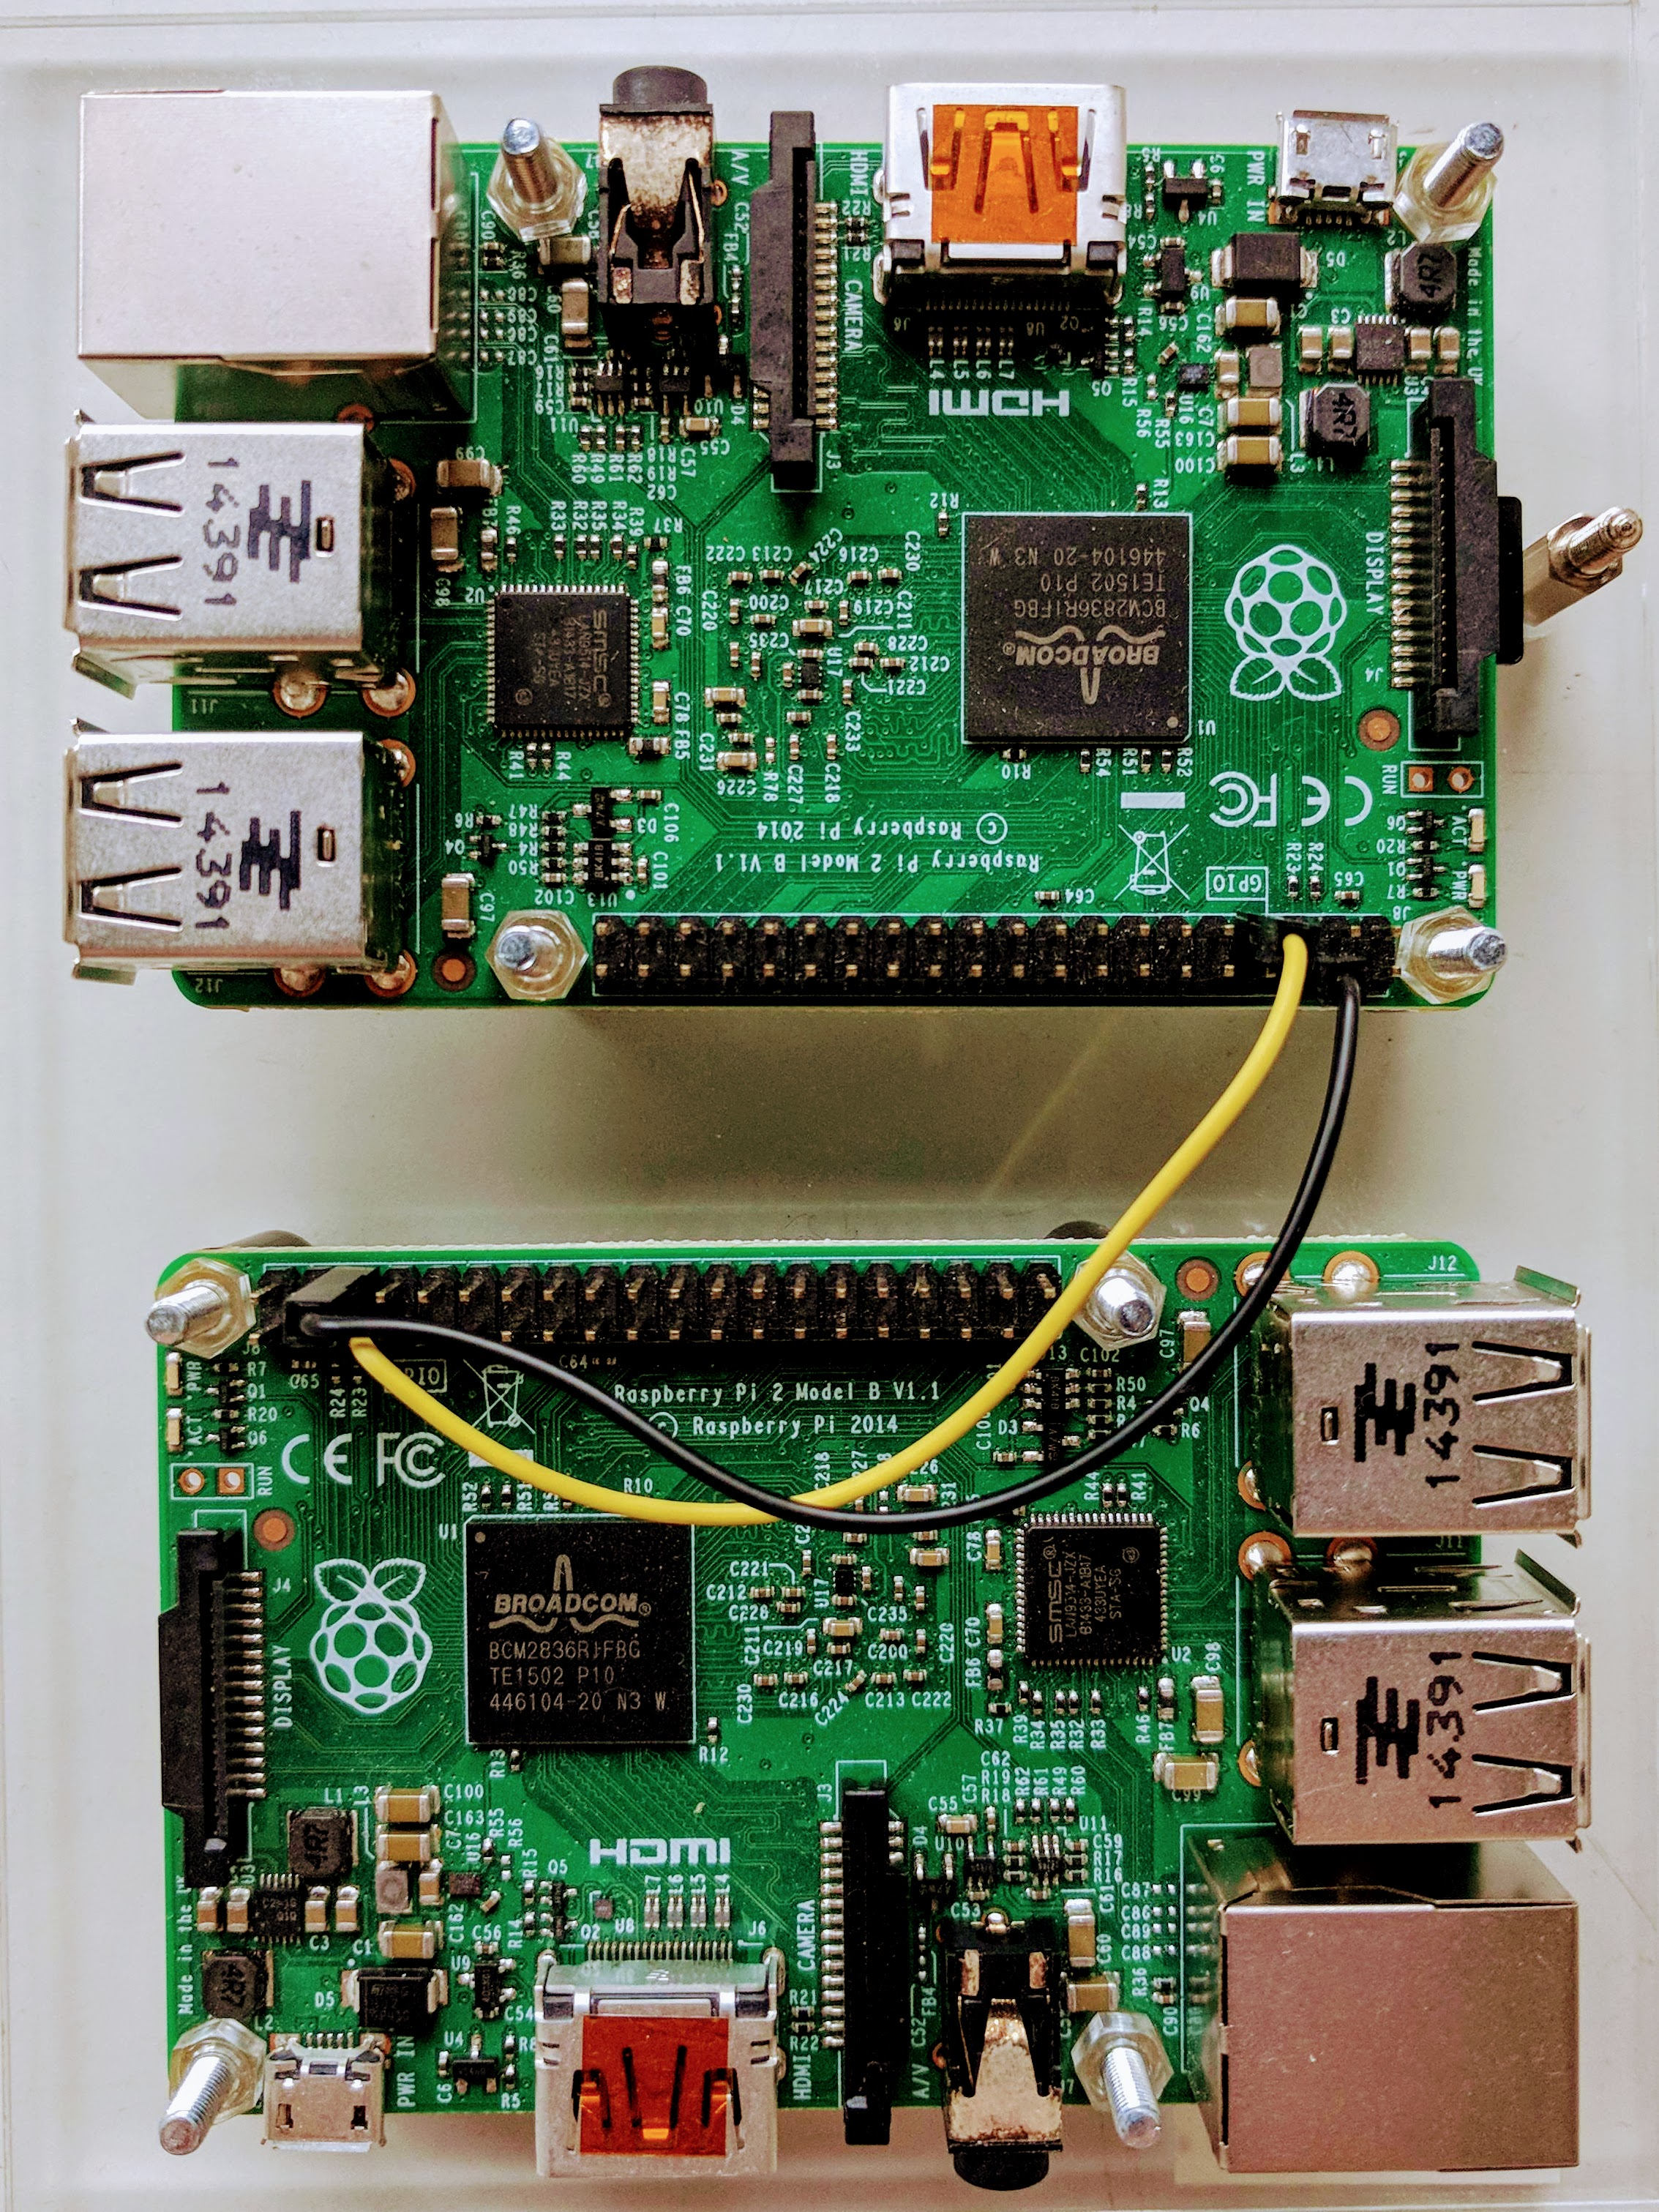
\includegraphics[width=0.35\textwidth]{gfx/raspi_board.jpg}}
	\caption{Das Raspi Loan-Board }
	\label{fig:click}
\end{wrapfigure}
Die vorliegende Arbeit beschäftigt sich mit der Einwicklung einer Datenbank-Applikation für das PSE-Labor\cite{website:17}, das sich an der Beuth Hoschschule für Technik Berlin befindet und seit fast 5 Jahre ein wichtiger Teil des Studiums im Studiengänge Technische Informatik und Medieninformatik ist. Die zwei Mitaraber, Andreas Döpkens und Brian Schüler, beitragen selbstmotiviert zur den  Projekte, die zwar räumlich im PSE-Labor der Beuth-Hochschule sind und betrieben werden können\cite{website:1}, wurden aber als "das acaLab" genannt, bei dem es sich sozusagen um ein virtuelles Labor in einem reellen Labor handelt. Die acaLab-Projekte sollen als interessante Mitarbeiter-Beiträge neben den individuellen Tätigkeiten im Fachbereich 6 der Beuth-Hochschule bereichern und werden deshalb auch exemplarisch jedes Jahr auf der Langen Nacht der Wissenschaften gezeigt\cite{website:1}. An dieser Stelle ist auch noch anzumerken, die acaLab-Projekte aus den Mitteln des PSE-Labors finanziert werden und damit möglichst viele Studierende für lehr- und erkenntnisreichen Abschlussarbeiten eingeladen sind, de der Vergabe die Aufgaben aus den acaLab-Projekten als Abschlussarbeiten spart dem Fachbereich ein Budget. Die Erkenntnisse und Ergebnisse aus den acaProjekt-Tätigkeiten sind später in die Lehre einfließen zu lassen.\cite{website:1} Meine Abschlussarbeit widmet sich dem neuen Projekt des Labors namens "acaLoan-Raspi".

Während im PSE-Labor stattfindenden Übungsveranstaltungen im Studiengang Technische Informatik werden vorhandene im PSE-Labor die Raspberry Pi Minicomputers (kurz: Raspi)  an die Studierenden verliehen. Zu Beginn einer Laborübung werden die Raspi Boards den Studierenden vom Lehrkraft, der die Übung betreut, übergeben und am Ende der Laborübung zurückgezogen. Aus 16 vorhandenen im Labor Raspis, die markierte mit den Nummern 12-16 von Studierenden nach Hause (home-loan) genommen werden können.\cite{website:1} 

Nachweislich ist das Vorgehen oft mit Reihe von Problemen verknüpft, die sich jedes Semester und fast jedes Mal wiederholen. Die folgenden Problemen wurden von Mitarbeitern des Labors bereits festgestellt und regelmäßig verlangsamen den Prozess der Verleihung und Übungsführung: 
\begin{itemize}
	\item Studierende kennen ihre am Semesteranfang zugewiesene Gruppennummer auch nach mehreren Wochen nicht und geben den Lehrkraft einen Board mit einer falschen Registriernummer, der einer anderen Gruppe früher zugewiesen wurde und nur von der zugewiesenen Gruppe benutzt werden darf. 
	\item Studierende versuchen  einen Board nach Hause auszuleihen, der zu den Lab-Boards gehört und nur im Labor während der Übungszeit verliert werden darf. Außerplanmäßig von Studierenden darf Lab-Board nicht ausgeliehen und auch mit nach Hause (home-loan) nicht genommen werden.
	\item Es gibt ein Verwaltungsaufwand für die ausleihbaren Home-Boards, die von den Studierenden für jeweils eine Woche mit nach Hause genommen werden können. Die Mitarbeiter müssen handlich die Studentenname, Matrikelnummer, Board und Zeit am Zettel registrieren und in einer Woche überprüfen, ob alle ausgeliehenen Boards pünktlich ins Labor zurückgekommen sind. 
	\item Erfahrungsgemäß können Studierende nach Ablauf der Frist ein Ausleihgerät in einem sehr üblen Zustand der Verschmutzung oder Zerstörung zurückgeben, dass es besteht eine Notwendigkeit den Zustand des Gerätes stets zu kontrollieren, damit es immer bekannt wird, zum welchen Zeitraum Raspi Board zum letzten Mal funktionsfähig war und von wem ausgeliehen wurde.  
	\item Falls gilt ein Raspi Board als verloren, es sollte eine Möglichkeit geben, alle vorherigen Ausleihen anzuschauen und festzustellen, von welchem Studierende es ausgeliehen und nicht zurückgegeben wurde. Mit den Zettelchen, auf denen einen Name von Studierende und eine Board Nummer gemerkt werden, ist es zu aufwändig nachvollziehen.	
\end{itemize}

Somit ist schlusszufolgern, dass eine Notwendigkeit das Verleihprozedere für die Loan-Boards (Lab und Home) mit modernen Mitteln der Technischen Informatik zu lösen schon dringend besteht und eine lohnenswerte Aufgabe für zukünftige Abschlussarbeit ist, schließlich aus drei Teilen bestehen wird:
\begin{itemize}
	\item Erstens wird an einem uComputer ein sogenannten Register-Client realisiert. Dafür ein RFID-Leser an uComputer angeschlossen wird. Register-Client ist neben dem Eingangstür eines kleinen Lagerraums des PSE-Labors zu platzieren ist, wo Raspi-Boards aufbewahrt werden. Es ist geplant, dass Studierende einen Board selbst aus dem Fach nehmen könnte und dann mit Hilfe des Register-Clients den genommenen Board auf sich oder seine Gruppe registrieren lassen. Der Register-Client hat selbst keinen Zugriff zur Datenbank und sollte nur die abgelesene Daten von der Smartcard der Studierende zur Server schicken. 
	\item Zweitens ist ein Display-Client zu entwickeln, der den Studierenden es zulässt, die Begrüßung des System und eine Beschreibung die für Ausleihe notwendigen Schritten zu sehen. Es sollte in einem Browser-Fenster die aktuelle Server-Kommunikation und Auskunft angezeigt wird, ob die Ausleihe gelang oder ein Fehler aufgetreten war. Ein Android/iOS-Tablett ist eine gute Wahl für die technische Realisierung, da es die Kommunikation zwischen den Mensch und das System leicht und ohne erweiterte Hinweise zulässt. 
	\item Drittens ist ein Web-Server für die Datenbank-Applikation schließlich zu implementieren. Er umfasst alle Datensätze über die vorhandenen im Labor Raspi-Boards, registrierten zum Kurs Studierenden und die abgewickelten Leihvorgänge.  Web-Server wird mit einem Web-Framework Django erstellt. Django verfügt nun über die Funktionalität und Datenbasis, um die dafür erforderlichen Aktionen durchzuführen. Als Web-Framework bietet Django eine Reihe von Komponenten und Funktionen (Benutzerauthentifizierung, Hochladen von Dateien, Umgang mit Daten usw.), die bei jeder Webanwendungen benötigt werden. Mit einem Web-Framework muss ein Entwickler keine Zeit damit verschwenden, denselben Code von Grund auf neu jedes Mal zu schreiben.
\end{itemize}

Nachdem nun grundlegenden Funktionsweisen der Bestandteilen des Verteilten Systems geklärt sind, geht es zur Auswahl der Hardware. Der wichtigste Aspekt beim Hardwarekauf ist einerseits das vorhandene Budget des PSE-Labors und zum Anderen die Aufgaben, die zusammenspielenden Hardware erfüllen sollen. Zunächst müssen die 16 für die Ausleihe zur Verfügung stehenden Raspi Loan-Boards mit einem geeigneten RFID-Tag ausgestattet werden. Es ist selbstklebende NFC Tags zu verwenden, die klein und dünn sind und lassen sich auf der Rückseite des Schutzschirms zu befestigen und ein Aussicht und Funktionen des Geräts nicht zu beeinflussen. Es ist nicht unerwähnt zu lassen, dass Tags nicht ausgelesen werden können, wenn diese auf einen metallischen Gegenstand/Oberfläche geklebt wurden, da die Kommunikation aus physischen Gründen zwischen Tag und Lesegerät gestört werden kann. Die Raspi Loan-Boards sind mit einem Schutzschirm aus dem ein transparenter thermoplastischer Kunststoff geschützt und es wurde ins Labor getestet, dass die geklebte auf der Rückseite RFID-Tag lassen sich ablesen und den Board auf RFID Chip-Kartenleser zu platzieren. 

\section{Aufbau der Arbeit}
\label{sec:intro:themengebiet}
BLAAA 



 
 